\begin{figure}[t]
	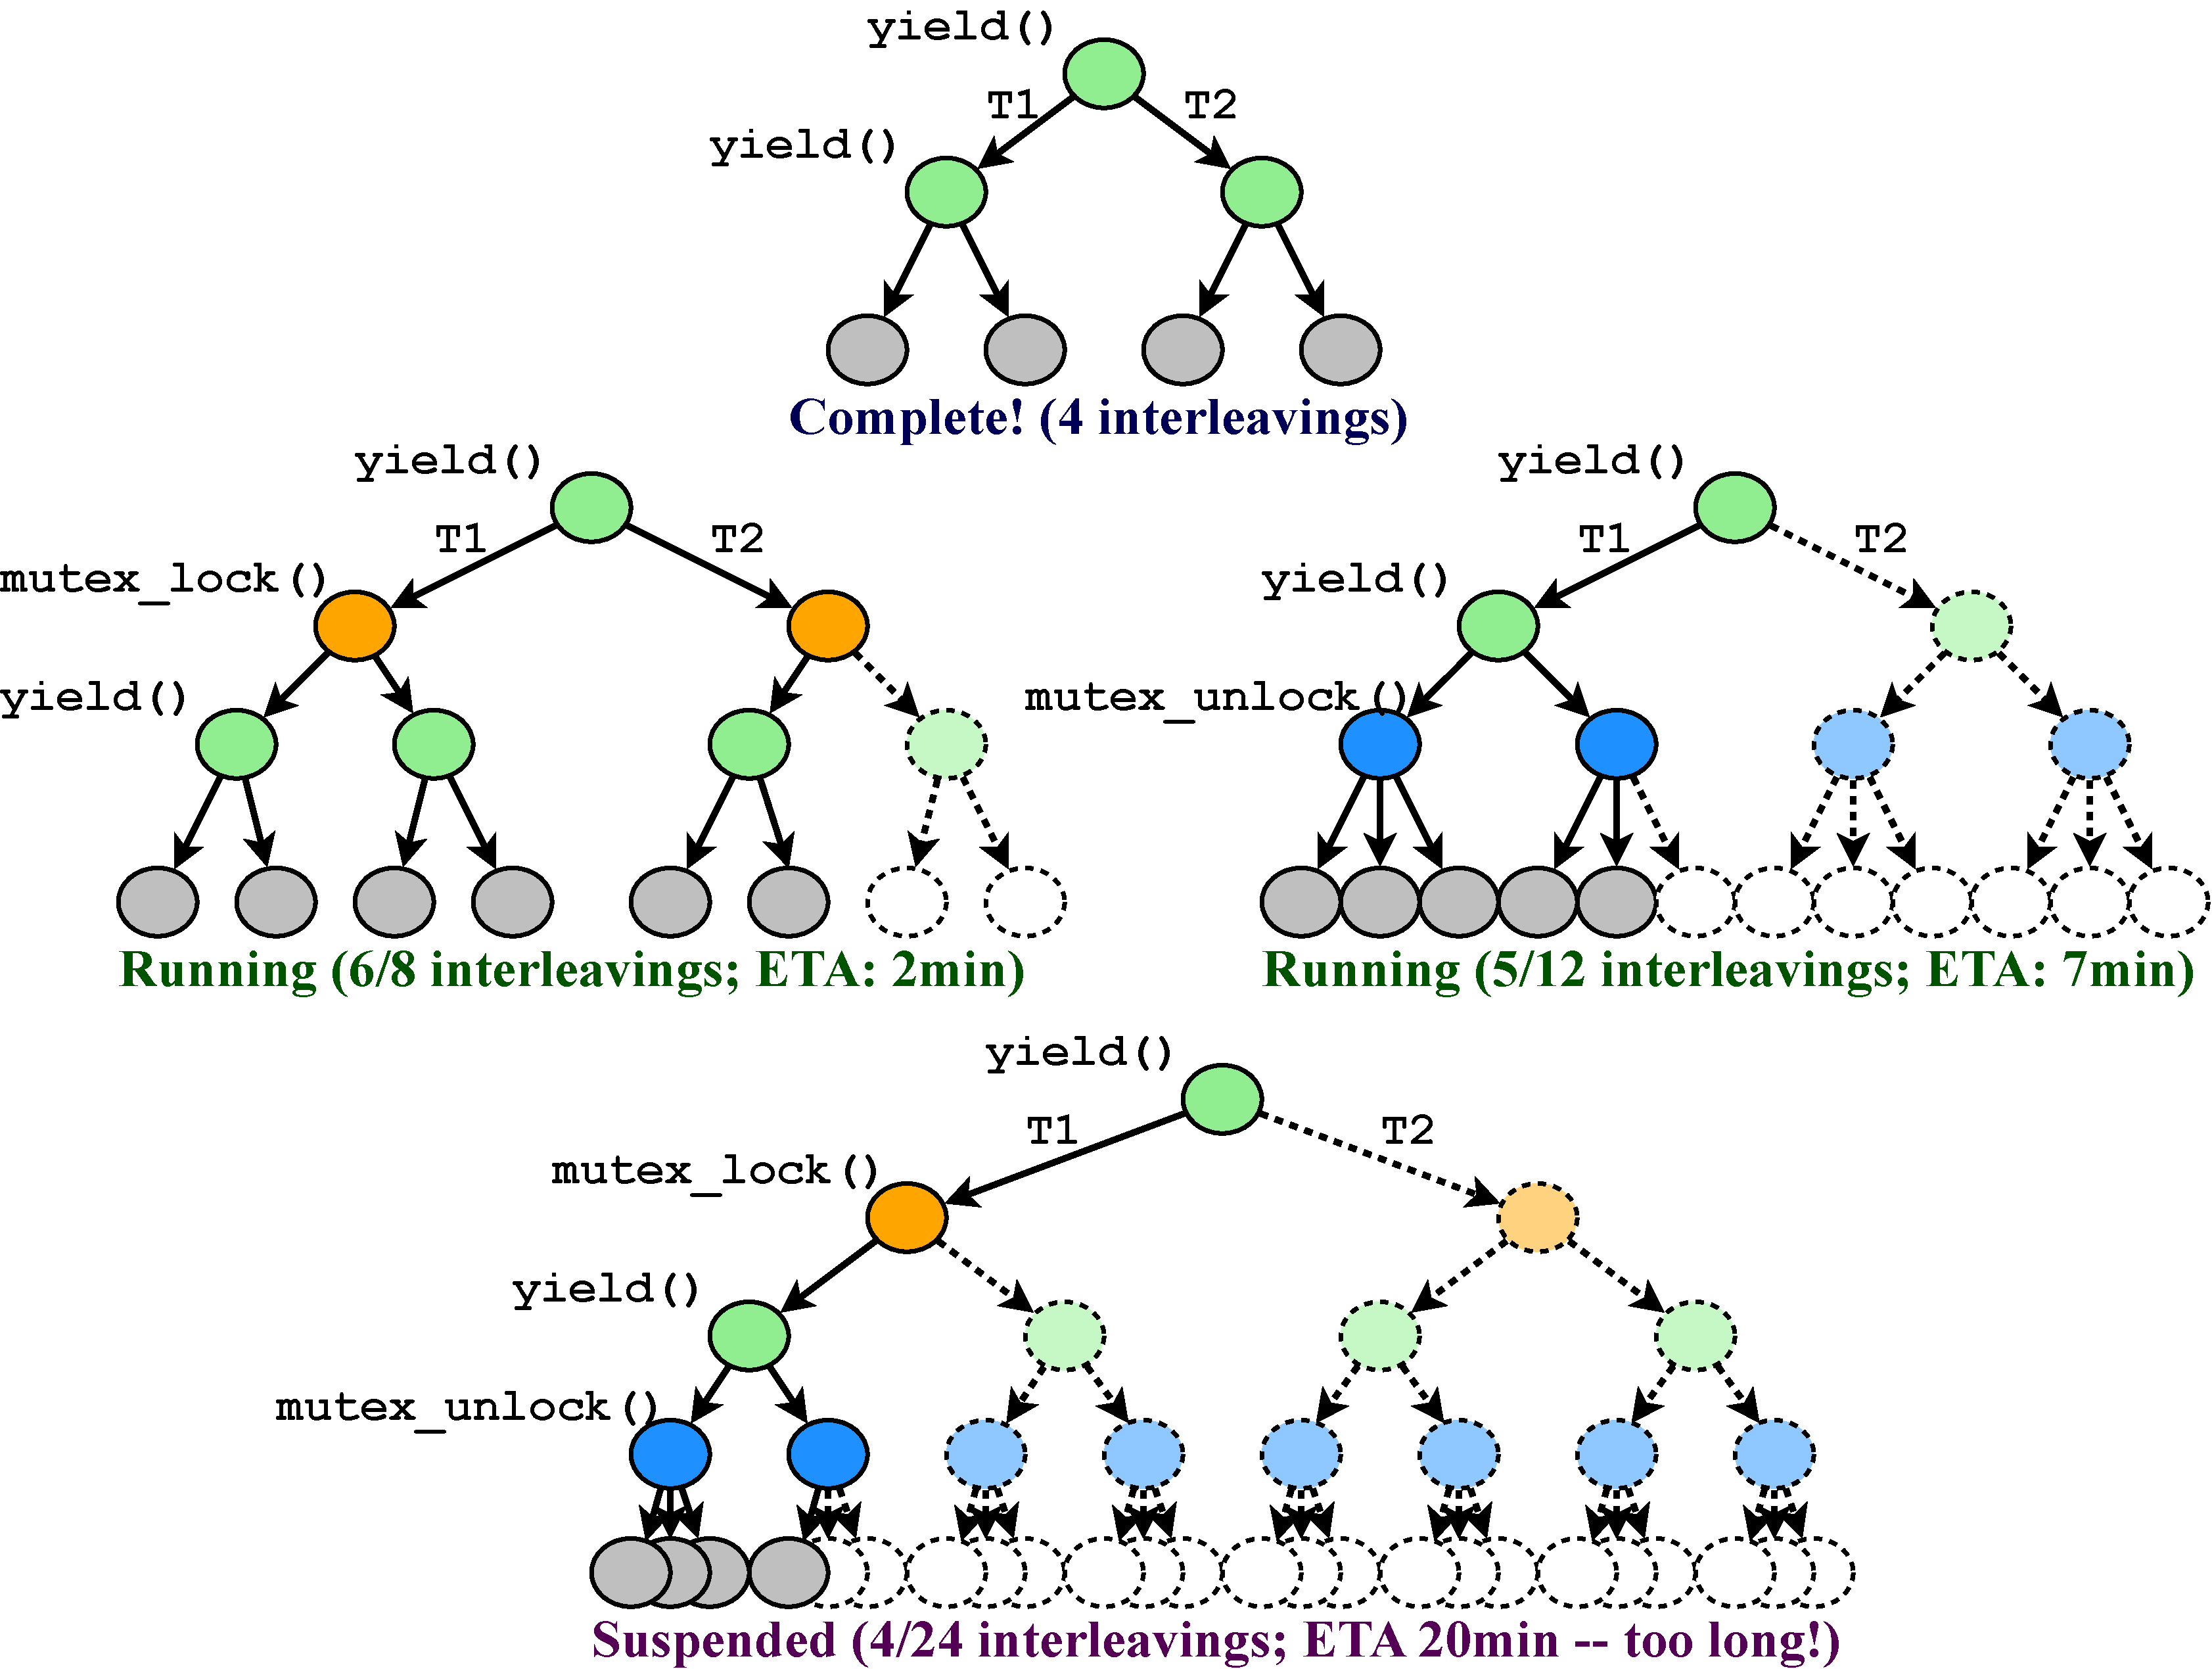
\includegraphics[width=0.48\textwidth]{trees.pdf}
	%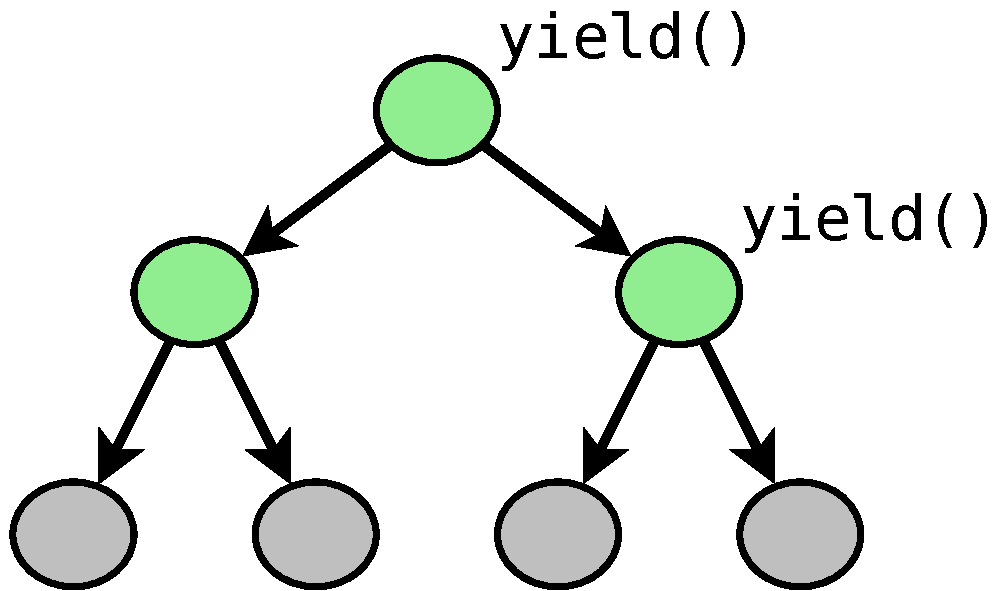
\includegraphics[width=0.15\textwidth]{tree0.pdf}
	%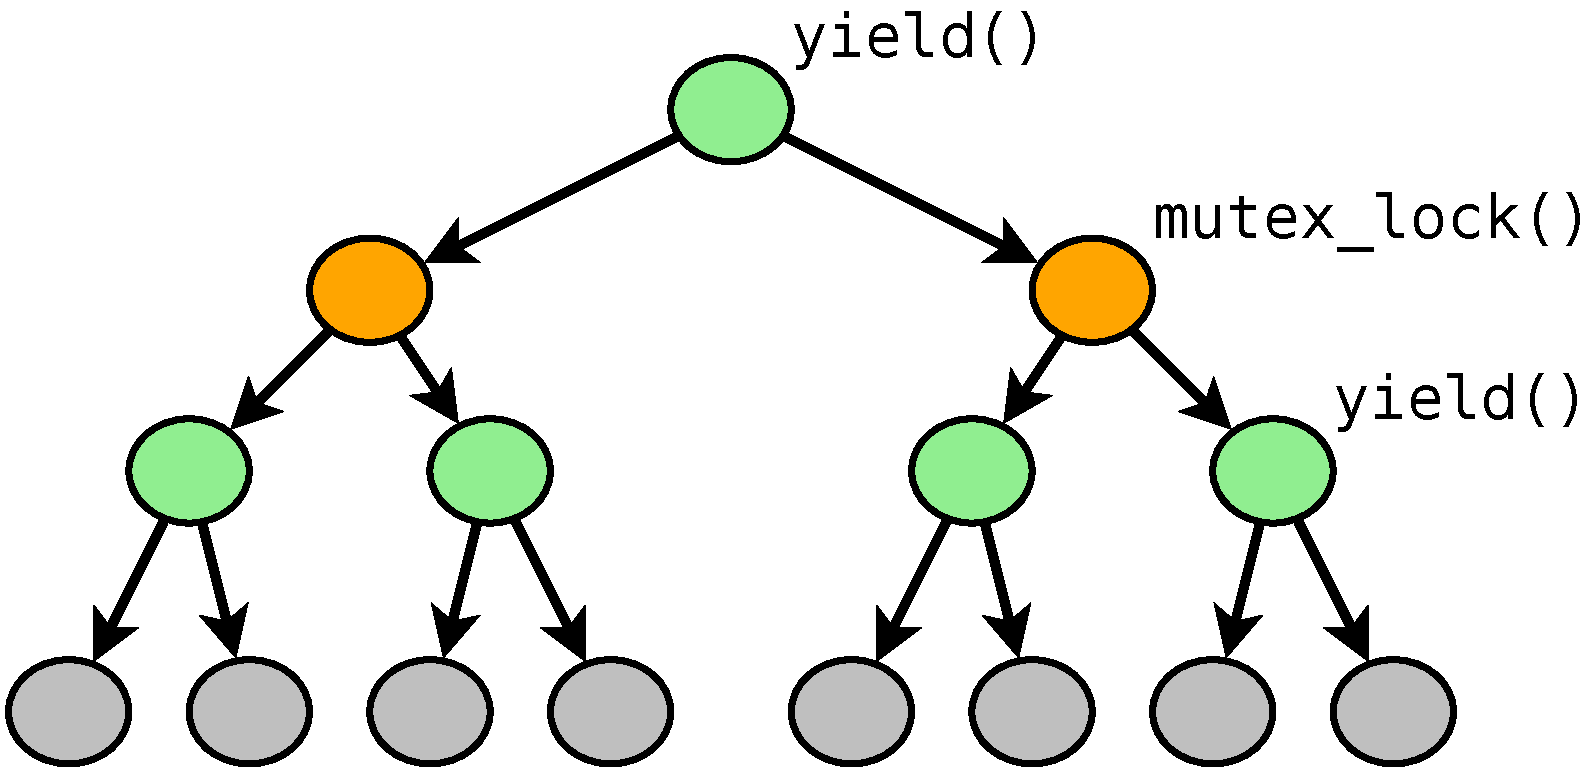
\includegraphics[width=0.225\textwidth]{tree1.pdf}
	%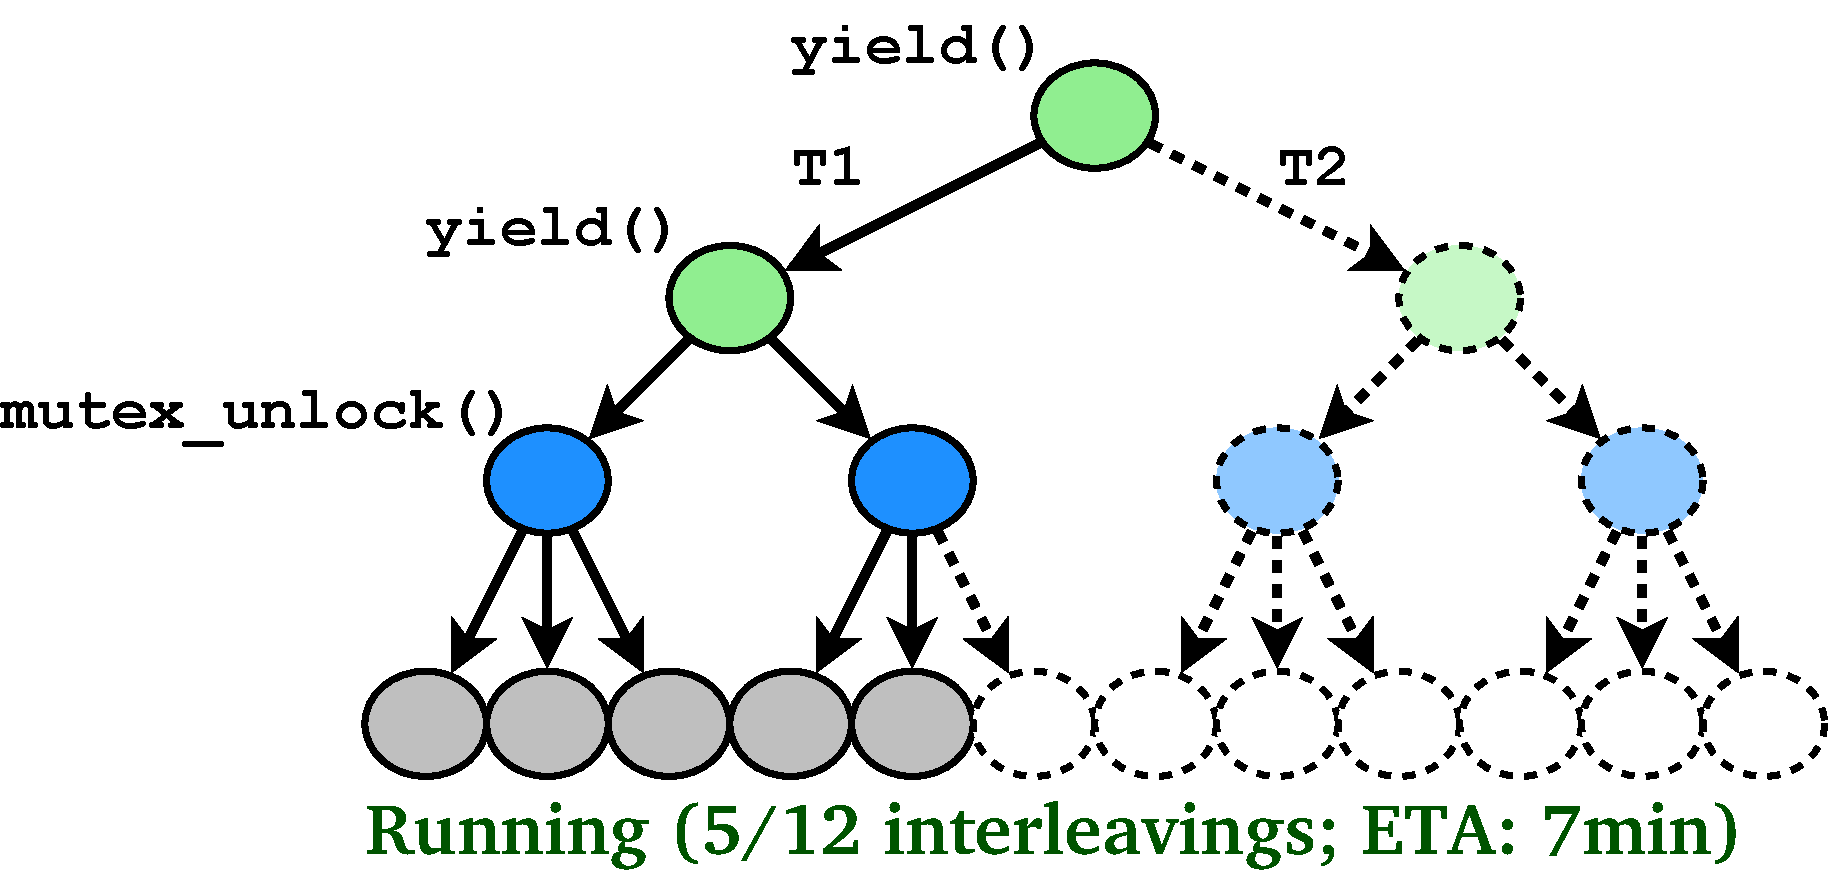
\includegraphics[width=0.25\textwidth]{tree2.pdf}
	%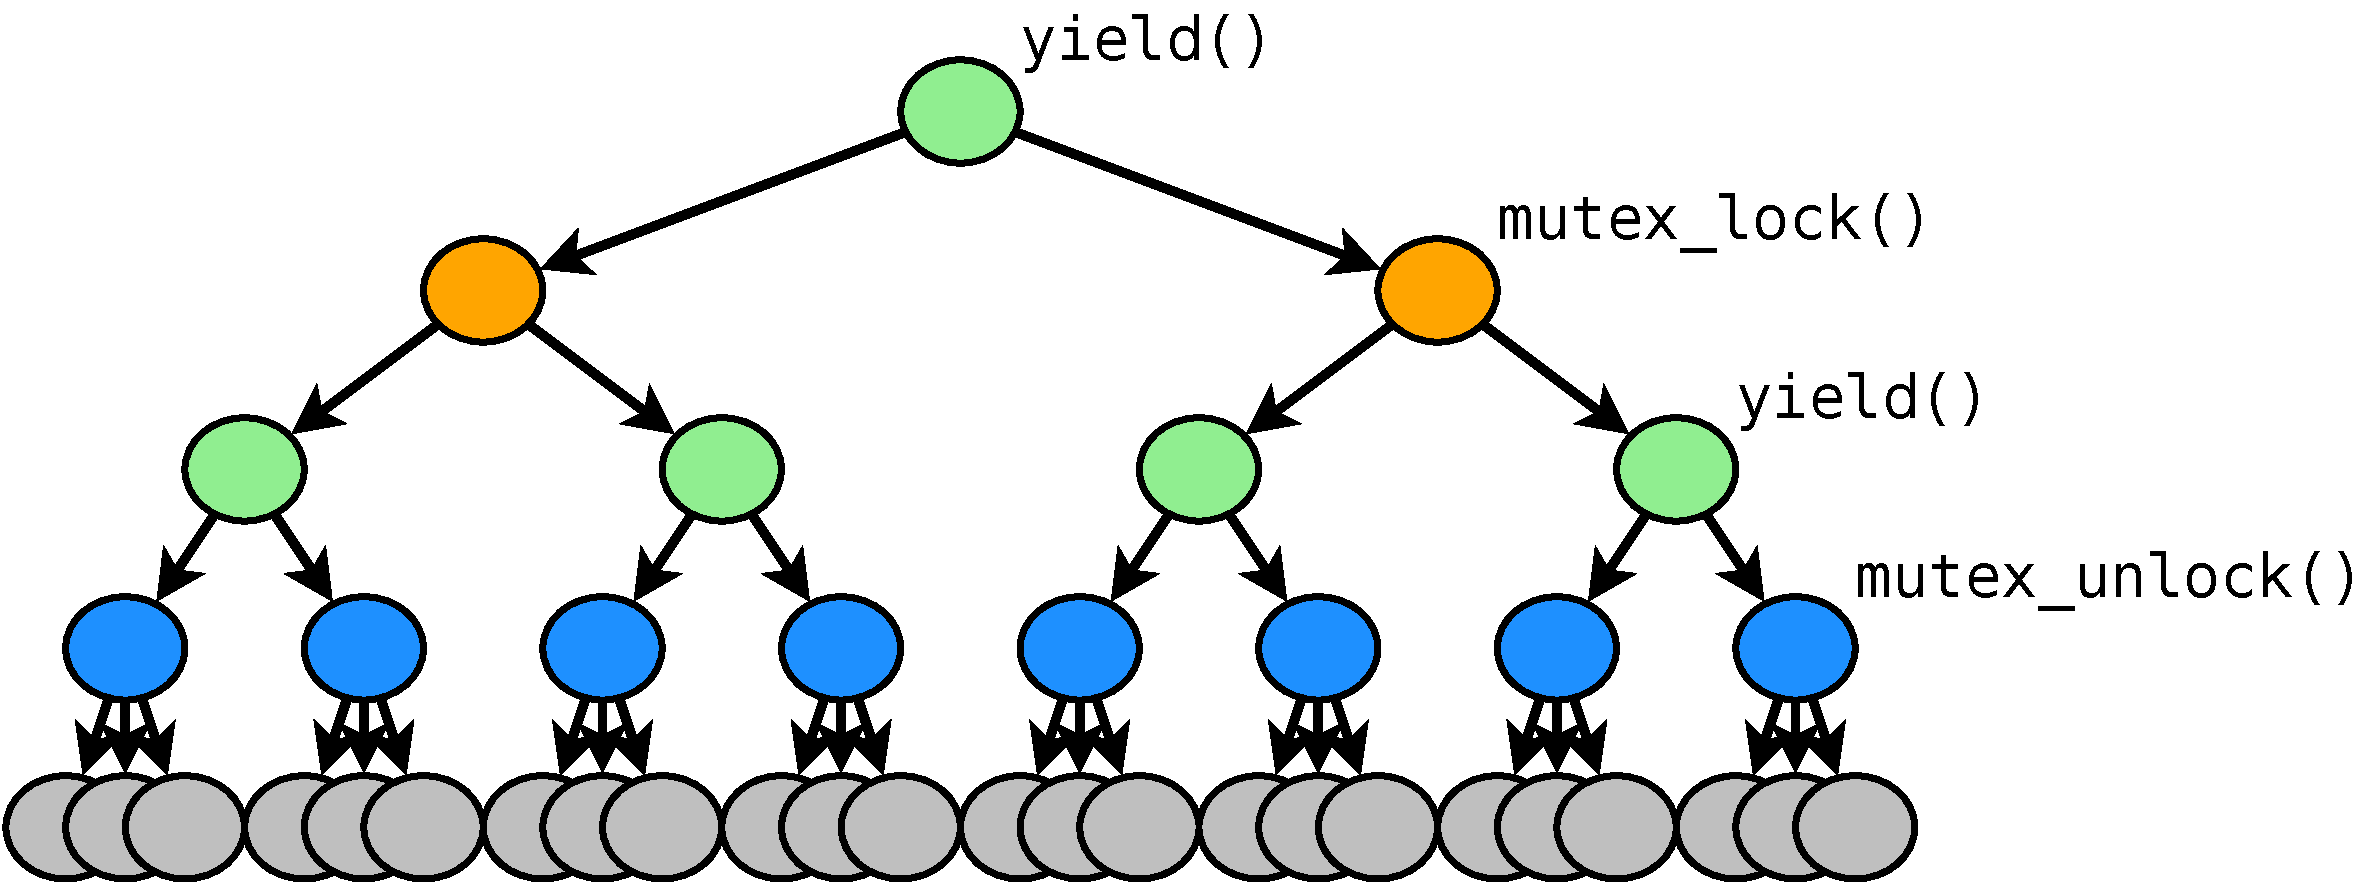
\includegraphics[width=0.35\textwidth]{tree3.pdf}
	\caption{Iterative Deepening example.
		The minimal state space (top) includes only voluntary thread switches, such as {\tt yield()} or {\tt cond\_wait()}~\cite{landslide}.
		Multiple further tests can be run: preempting on calls to {\tt mutex\_lock} alone (left), {\tt mutex\_unlock} alone (right), or both together (bottom).
Each option increases the state space size by an unpredictable factor, so multiple state spaces should be tested in parallel.
Estimation techniques~\cite{estimation} inform which state spaces to prioritize.
}
	\label{fig:id}
\end{figure}
\section{Design}

Motivated by state-of-the-art tools' inflexibility to change their preemption points,
Iterative Deepening searches among different combinations of such points during a test,
deciding on-the-fly whether to pursue each resulting state space or abandon it in favour of smaller ones.
Different state spaces are generated based on {\em subsets} of the preemption points which prior work would use; for example, ``preempt on all calls to {\tt mutex\_lock} but not on {\tt mutex\_unlock}.
We show a visualization in Figure~\ref{fig:id}.

Iterative Deepening depends heavily on state-space estimation \cite{estimation}
to understand which state spaces are likely to complete on time,
in advance of actually testing each interleaving within.
The purpose is to make decisions automatically about when to defer exploration of a state space,
so an inexpert user need only provide their total CPU budget as an argument,
and to enable completing appropriately-sized state spaces within that budget.

Note that Iterative Deepening is a {\em wrapper} algorithm around stateless model checking.
A model checking tool is still used to test each state space, and other reduction techniques are still applicable.
Moreover, because Iterative Deepening treats the set of preemption points as mutable,
it grants the potential to add new ones reactively based on any runtime analysis.
In this paper we focus on dynamic data-race detection~\cite{tsan} as the mechanism for finding new preemption candidates.

\subsection{Terminology}

For the remainder of the paper, we will abbreviate {\em preemption point} (PP),
{\em model checking} (MC),
{\em single-state-space model checking} (SSS-MC) (i.e., the approach of prior work),
and {\em state space estimate} (ETA).

Please note the difference between data-race {\em candidates} and data-race {\em bugs}.
Because data-race analysis is false-positive-prone,
we classify unprotected access pairs separately from concrete observable failures, % "concrete"?
calling such pairs {\em data race candidates}.
Should a future interleaving, preempting during those accesses, cause a failure (e.g. assertion or deadlock), then we report a {\em data-race bug}.
Otherwise, if the access pair can be reordered, but does not produce a failure under any interleaving, it is a {\em benign data race}.
If they cannot be reordered at all, it is a {\em false positive}.
For brevity, we count benign data races as a subset of false positives.

We also identify the {\em minimal} and {\em maximal state space} for each test.
The {\em minimal state space} includes only thread switches arising from normal execution (Figure~\ref{fig:id}).
The {\em maximal state space} is simply the one explored by SSS-MC: all statically-available PPs are enabled.
%However, should new data-race PPs be added during a test, the new maximal state space will be the one including those as well.

\subsection{Verifying data races as buggy or benign} % FIXME: dont say 'benign'; also, do you have enough left to say that this can even still be a full subsection?

\subsection{Choosing the best job}

% TODO: put colour in this code
\newcommand\PendingJobs{\ensuremath{\mathcal{P}}}
\newcommand\SuspendedJobs{\ensuremath{\mathcal{S}}}
\newcommand\GetETA[1]{ETA(#1)}
\newcommand\GetPPSet[1]{PPSet(#1)}
\begin{algorithm}[t]
	\SetKwInOut{Input}{Input}
	%\textbf{Function} GetBestJob($j_0$, PendingJobs, SuspendedJobs): \\
	\Input{$j_0$, the currently-running job}
	%\Input{$eta$, $j_0$'s predicted completion time}
	\Input{\PendingJobs, the list of pending jobs, sorted decreasingly by heuristic priority}
	\Input{\SuspendedJobs, the list of already-suspended jobs, sorted increasingly by ETA}
	\If{\GetETA{$j_0$} $<$ HeuristicETAFactor $\times$ TimeLeft()}{
		// common case: job will probably finish on time \\
		return $j_0$
	}
	\ForEach{job $j_P \in$ \PendingJobs}{
		// don't run a pending job if a subset of it is already suspended; it would find the same fate! \\
		\If {$\forall j_S \in$ \SuspendedJobs, \GetPPSet{$j_S$} $\not\subset$ \GetPPSet{$j_P$}}{
			return $j_P$
		}
	}
	%// no pending jobs; maybe resume a suspended job \\
	\ForEach{job $j_S \in$ \SuspendedJobs}{
		\If{\GetPPSet{$j_0$} $\not\subset$ \GetPPSet{$j_S$}
			$\land$
			\GetETA{$j_0$} $>$ \GetETA{$j_S$}}{
			// $j_S$ is tempting, but if a subset of it is also suspended, don't run the larger one first \\
			\If{$\forall j_{S2} \in$ \SuspendedJobs, \GetPPSet{$j_{S2}$} $\not\subset$ \GetPPSet{$j_S$}}{
				return $j_S$
			}
		}
	}
	// $j_0$'s ETA was bad, but nothing else was better \\
	return $j_0$
	\caption{Suspending exploration of a too-large state space in favour of a potentially smaller one.}
	\label{alg:shouldworkblock}
\end{algorithm}

With a limited CPU budget, we must avoid running tests likely to time out.
When a MC instance reports too high ETA (greater than some heuristic factor times the time remaining),
we compare other yet-untested PP sets to find another job more likely to complete in time.
This algorithm is the heart of Iterative Deepening; we list it in Algorithm~\ref{alg:shouldworkblock}\footnote{
Though its worst-case performance is $O(mn)$ in the number of pending and suspended jobs,
in practice the non-constant portion runs very infrequently
and is negligible compared to the exponentially-sized state spaces.}.
The algorithm takes into account... TODO

% TODO: should work block / find work algorthm here

%%%%%%%%%%%%%%%%%%%%%%%%%%%%%%%%%%%%%%%%%%%%%%%%%%%%%%%%%%%%%%%%%%%%%%%%%%%%%%%%

\section{Implementation}

\subsection{Landslide}
\label{sec:landslide}

We chose \landslide~\cite{landslide} as our stateless model checker due to its ability to trace program execution at the granularity of individual instructions and memory accesses, which is mandatory for dynamic data-race analysis.
\landslide~features Dynamic Partial Order Reduction (DPOR) \cite{dpor}, state space estimation, and hybrid lockset/happens-before data-race detection.
It avoids state space cycles (e.g. ad-hoc synchronization with {\tt yield()} or even {\tt xchg} loops) with a heuristic similar to Fair-Bounded Search \cite{bpor}. % TODO: devote a paragraph to this, after talking about drs in locks
% this line can be cut if space is needed
It can test both user- and kernel-level code, although is limited to timer-driven nondeterminism.
Its bug-detection metrics include assertion failure, deadlock, segfault, heap checking (like Valgrind~\cite{valgrind}), and a heuristic infinite loop/livelock check.

{\bf Restricting PPs with stack trace predicates.}
Most MCs preempt indiscriminately on any sync API call, regardless of the call-site.
However, when testing a particular module in a large codebase,
the user is likely uninterested in PPs arising from other modules.
\landslide~provides the {\tt within\_function} configuration command for a user to identify which call-sites matter most.
Before inserting a PP, \landslide~requires at least one argument to {\tt within\_function} to appear in the current thread's stack trace.
The {\tt without\_function} directive works similarly, but as a blacklist.
Multiple invocations can be used; later ones take precedence.
%\cite{landslide} provides further detail on this feature.

{\bf Data races in lock implementations.}
Prior work data race tools recognize the implementations of sync primitives to avoid spuriously flagging memory accesses resulting from the lock implementation itself \cite{tsan}.
Assuming the locks are already correct enables productive data-race analysis on the rest of the codebase.
With testing limited to one execution, even if you wished to test for lock bugs, data-race analysis would still uselessly flag every single access pair in the lock implementation, requiring human attention to verify.
However, Iterative Deepening can automatically verify a large quantity of data-race candidates as benign.
Hence, we extended \landslide~with a custom option to change the lock-set tracking to include accesses from {\tt mutex\_lock()} and {\tt mutex\_unlock()} in the analysis. (Accesses from other sync functions, such as {\tt cond\_wait()}, would be either included already, or protected by an internal mutex.)
% TODO: Add a code sample showing how the lockset boundaries change? If there's room?

\subsection{Quicksand} %Managing multiple state spaces

\quicksand~is an independent program that wraps the execution of several \landslide~instances.
The implementation is roughly 3000 lines of C code.



\quicksand~uses a workqueue model
...
priorities... data race priorities...

{\bf Communication protocol.}
The interface to \landslide~, which any similar MC could implement, is in two parts.
First, when starting each job, it writes a configuration file declaring which PPs to use,
% can lose this line due to space
among other options such as mutex-testing mode,
passed as an argument to \landslide.
Then, a dedicated \quicksand~thread communicates with the \landslide~process via message-passing on a FIFO pipe.
\landslide~sends a message after each new interleaving is tested, to report updated progress and ETA,
whenever a new data-race candidate is found, and whenever a bug is found.
\quicksand~in turn replies whether the test should suspend/resume due to too high ETA, or quit due to timeout.

{\bf Heuristics.}


% If there's room, mention the cant_swap mechanism for killing the top half of deferred jobs.

{\bf Avoiding thrashing in \quicksand.} % TODO

% TODO: decide which subsection should come first for better flow

\subsection{Data-race preemption points}

% Intuitively, % TODO describe what we're trying to achieve % do this in design section

When \landslide~detects a data race, it reports each of the two memory accesses involved in the race.
Each report indicates the program counter value (PC) associated with the access, as well as some further conditions to help filter away unrelated executions of the same instruction on different data.
(For example, {\tt list\_insert()} might be called from many parts of a codebase, but produce data-race candidates from only one callsite.)
Ideally, the PC would be qualified by a full backtrace, but tracing the stack is too expensive to do for each shared memory access.
Instead, \landslide~qualifies the PC with
(a) the current thread ID and
(b) the most recent {\tt call} instruction.
% (a crude approximation of a stack trace)
% which are much cheaper, as we carry them around all the time already
Note that we do {\em not} qualify data races by the shared memory address,
which can change based on different interleavings of previous code
(for example, depending on the result of {\tt malloc()}).
% especially when malloc is involved.
% TODO: decide whether to make dont-filter-dr-by-address example.
%Figure~\ref{fig:dont-filter-dr-by-address} shows example code where qualifying by memory address will miss the bug.


When \quicksand~receives a data race report, it adds two new jobs to its workqueue:
a ``small'' job to preempt on the racing instruction only,
and a ``big'' job to preempt on that instruction as well as each PP used by the reporting job.
%
Hence each {\em pair} of racing accesses will spawn four new jobs, as shown in Figure~\ref{fig:new-dr-jobs}.
Rather than adding a maximal job with both new PPs at once, we prefer to add smaller jobs which have a higher chance of completing in time.
If those state spaces are bug-free, they will in turn add the maximal job later.
%
The rationale of spawning multiple jobs is that which will be more fruitful cannot be known in advance:
while the big job risks not completing in time,
the small job risks missing the data race entirely if the original PPs were required to expose it.
In practice, we observed some bugs found quickly by these small jobs, and other bugs missed by the small jobs found eventually by the big jobs,
which motivates the need for Iterative Deepening to decide at runtime which to prioritize.
% TODO: Put numbers here.
% which justifies this design


% TODO: make new-dr-jobs diagram

%                                  (2)          landslide         landslide
%  landslide                   "Preempt when-->  o  PPs=[foo]      o  PPs=[mutex_lock,
%    o  PPs=[mutex_lock]        PC = FOO"       / \               / \      foo]
%   / \                              |         o   o             o   o
%  o  /\                             |                          /|\  |\
%    o  o                                                      o o o o o
%                             __QUICKSAND__
%    |       (1)             |             |           (3)
%    \  "Hey, an access      |  job1       | ----"Preempt when -->
%     '- at FOO raced w/ --> |        job2 |      PC = BAR"
%        one at BAR!         |    job4     |
%                            |        job70|      [ same pictures for s/foo/bar/]
%                            | job8        |
%                            '-------------'
%                maybe show some internal structore of QS as well

% TODO: Decide whether to discuss the fact that we don't add the 2nd of a "suspected" dr pair until it is confirmed.

\subsection{Suppressing ``malloc-recycle'' false positives}
\label{sec:recycle}

% TODO: Understand what prior work means by 'happens before'. It's different from our MUST happen before relation.
% TODO: Understand how it relates to this. Would it scoop us? Or are we outside their model?

We identify a particular class of false positive data-race candidate in which the associated memory is recycled by {\tt malloc} between the two accesses.
Figure~\ref{fig:recycle} shows a common code pattern and interleaving which can expose such behavior.
If the {\tt malloc} on line 4 returns the same address passed to {\tt free} on line 2, then lines 1 and 7 will be flagged as a data race.
We term this a {\em malloc-recycle data race}.
To the human eye, this is obviously a false positive: reordering lines 4-7 before lines 1-2 will change {\tt malloc}'s return value, causing {\tt x} and {\tt y} to no longer collide.
Here, Thread 2's logic usually corresponds to the initialization pattern \cite{eraser}, but for generality we have added a {\tt publish} action on line 6.

\begin{figure}[t]
	\small
\begin{tabular}{rll}
	& \multicolumn{2}{c}{\texttt{struct x \{ int foo; int baz; \} *x;}} \\
	& \multicolumn{2}{c}{\texttt{struct y \{ int bar; \} *y;~~~~~~~~~~}} \\
	\\
	& Thread 1 & Thread 2 \\
	1 & \texttt{\hilight{brickred}{x->foo = ...;}} & \\
	2 & \texttt{\hilight{olivegreen}{free}(x);} \\
	3 & & \texttt{// x's memory recycled} \\
	4 & & \texttt{y~=~\hilight{olivegreen}{malloc}(sizeof *y);} \\
	5 & & \texttt{// ...initialize...}\\
	6 & & \texttt{publish(y);} \\
	7 & & \texttt{\hilight{brickred}{y->bar = ...;}} \\
\end{tabular}
\caption{A common execution pattern with {\tt malloc()} that produces false positive data race candidates.}
\label{fig:recycle}
\end{figure}

% This class of false positive is unique to heap-allocated memory, among all ways threads could communicate. By contrast, global memory has unlimited lifetime, and message-passing primitives enforce a must-happens-before relationship which precludes the race.

It is quite simple to mechanically recognize when {\tt x} and {\tt y} correspond to different abstract allocations despite colliding on address.
\landslide~implements this check by adding a generation counter to its heap state tracking:
each allocation is given a unique ID,
and when evaluating whether two heap accesses can race,
the IDs of their containing blocks must match.
However, when limited to a single execution, suppressing any data race matching this pattern is unsound.
Consider the more unusual program in Figure~\ref{fig:recycle-bug}:
Now, the memory is recycled the same way, but the racing access's address is not tied to {\tt malloc}'s return value.
Hence, reordering lines 6-7 before line 3 will cause {\tt x} and {\tt x2} to race.

\begin{figure}[t]
	\small
\begin{tabular}{rll}
	& Thread 1 & Thread 2 \\
	1 & \texttt{publish(x);} & \\
	2 & & \texttt{x2 = get\_published\_x();} \\
	3 & \texttt{\hilight{brickred}{x->foo = ...;}} & \\
	4 & \texttt{\hilight{olivegreen}{free}(x);} \\
	5 & & \texttt{// x's memory recycled} \\
	6 & & \texttt{y~=~\hilight{olivegreen}{malloc}(sizeof *y);} \\
	7 & & \texttt{\hilight{brickred}{x2->foo = ...;}} \\
\end{tabular}
\caption{If a single-pass data race detector discarded candidates matching the malloc-recycle pattern,
it would miss the bug in this adversarial program.}
\label{fig:recycle-bug}
\end{figure}

% TODO: Figure out why they claim "Happens before produces NO false positives, only benign races".
% It seems impossible.
% But if true, it means either (a) they can somehow identify FRM DRs on the 1st pass, not needing to replay,
% or (b) reuse of memory by malloc is somehow outside their concurrency model.

% TODO: proof goes here
% TODO: example codez with malloc re free go here
